%!TEX root = ../../main.tex

\chapter{Das Monty-Hall-Problem - Einführung}

Das Monty-Hall-Problem ist Statistikern als Paradoxon in der Elementarwahrscheinlichkeitstheorie bekannt. Es geht dabei um die Frage, ob eine Wahl, die zunächst 
zufällig unter drei \footnote[1]{a priori} gleich wahrscheinlichen Möglichkeiten getroffen wurde, geändert werden sollte, wenn zusätzliche Informationen enthüllt werden.
Die Aufgabe ist ursprünglich aus der von Monty Hall modertierten Spielshow "Lets Make a Deal" abzuleiten.


% \begin{figure}[h]
% \centering
% 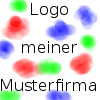
\includegraphics[height=.8\textwidth]{logo.png}
% \caption{Das Logo der Musterfirma\footnotemark}
% \end{figure}



%\begin{wrapfigure}{r}{.4\textwidth}
%\centering
%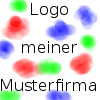
\includegraphics[height=.35\textwidth]{logo.png}
%\vspace{-15pt}
%\caption{Das Logo der Musterfirma\footnotemark}
%\end{wrapfigure}
%Quelle muss in Fußnote stehen (da sonst aufgrund eines Fehlers nicht kompiliert
% wird)
\footnotetext{aus \cite{mustermann:2012}}


% \begin{equation}
% t-t_{0}=\sqrt{\frac{l}{g}}\int_{0}^{\varphi}{\frac{d\psi}{\sqrt{1-k^{2}\sin^{2} {\psi}}}} = \sqrt{\frac{l}{g}} F(k,\varphi)
% \label{xyz}
% \end{equation}

% \begin{itemize}
% \item Dies ist der erste Punkt, der aufgeführt wird.
% \item Dies ist der zweite Punkt, der aufgeführt wird. Manchmal will man auch etwas \textbf{fett} oder \textit{kursiv} oder \textbf{\textit{beides in Kombination}}  drucken.
% \item Dies ist der dritte Punkt, der aufgeführt wird.
% \end{itemize}


Verweise auf das Glossar: \gls{Glossareintrag}, \glspl{Glossareintrag}

